% ft-09-BasicDiff.tex

\documentclass[xcolor=dvipsnames]{beamer}

\usepackage{cancel}
\renewcommand{\CancelColor}{\color{red}}
\usepackage{graphicx}
\usepackage{wrapfig}
\usepackage{colortbl}
\usepackage{color}
\usepackage{alltt}
\renewcommand*{\thefootnote}{\fnsymbol{footnote}}
\definecolor{myblue}{rgb}{0.8,0.85,1}

\mode<presentation>
{
  \usetheme{Warsaw}
  \setbeamercovered{transparent}
}
% \usecolortheme[named=OliveGreen]{structure}
\setbeamertemplate{navigation symbols}{} 
\setbeamertemplate{blocks}[rounded][shadow=true] 

% this is for overlaying math symbols, see https://tex.stackexchange.com/questions/12895/overlay-symbol-with-another
\def\qeq{\mathrel{%
    \mathchoice{\QEQ}{\QEQ}{\scriptsize\QEQ}{\tiny\QEQ}%
}}
\def\QEQ{{%
    \setbox0\hbox{$\longrightarrow$}%
    \rlap{\hbox to \wd0{\hss/\hss}}\box0
  }}

\newcounter{expls}
\setcounter{expls}{0}
\newcommand{\beispiel}[1]{\refstepcounter{expls}\textbf{Example \arabic{expls}: #1.}}

\newcounter{exercise}
\setcounter{exercise}{0}
\newcommand{\ubung}[0]{\refstepcounter{exercise}\textbf{Exercise \arabic{exercise}: }}

\newif\ifBCITCourse
\BCITCoursetrue
% \BCITCoursefalse
\newif\ifWhichCourse
\WhichCoursetrue
% \WhichCoursefalse
\ifBCITCourse
\ifWhichCourse
\newcommand{\CourseName}{Technical Mathematics for Food Technology}
\newcommand{\CourseNumber}{MATH 1441}
\newcommand{\CourseInst}{BCIT}
\else
\newcommand{\CourseName}{Technical Mathematics for Geomatics}
\newcommand{\CourseNumber}{MATH 1511}
\newcommand{\CourseInst}{BCIT}
\fi
\else
\newcommand{\CourseName}{Philosophy and Literature}
\newcommand{\CourseNumber}{PHIL 375}
\newcommand{\CourseInst}{UBC}
\fi

\title{Basic Rules of Differentiation}
\subtitle{{\CourseNumber}, BCIT}

\author{\CourseName}

\date{October 18, 2017}

\begin{document}

\begin{frame}
  \titlepage
\end{frame}

\begin{frame}
  \frametitle{Functions}
A \alert{function} is a rule that assigns to each element in a set $A$ one and
only one element in a set $B$.

\medskip

\emph{Exercise:} Find the maximum domain and range of the following
functions on the real number line:
\begin{equation}
  \label{eq:sijoomai}
  f(x)=\sqrt{x-1}
\end{equation}
\begin{equation}
  \label{eq:vooghahk}
  f(x)=\frac{1}{x^{2}-4}
\end{equation}
\begin{equation}
  \label{eq:zaekohxi}
  f(x)=x^{2}+3
\end{equation}
\end{frame}

\begin{frame}
  \frametitle{Function Graphs}
The \alert{graph of a function} $f$ is the set of all points $(x,y)$
in the $xy$-plane such that $x$ is in the domain of $f$ and $y=f(x)$.
  \begin{figure}[h]
    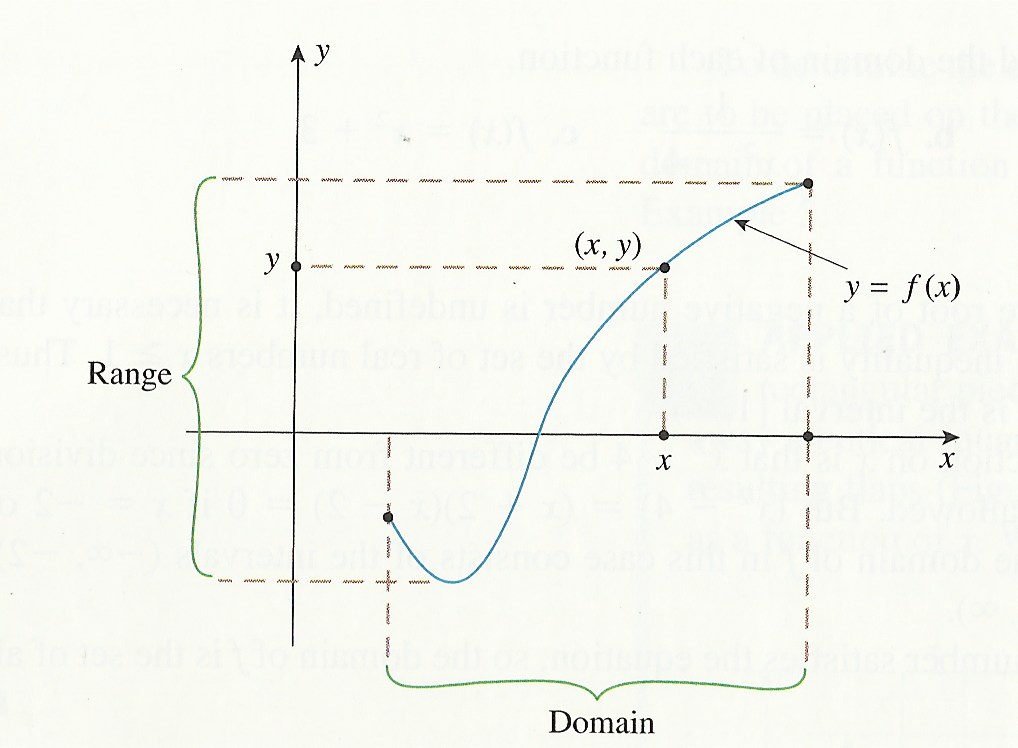
\includegraphics[scale=1]{./fgraph-02.png}
  \end{figure}
\end{frame}

\begin{frame}
  \frametitle{Vertical Line Test}
Every function $f$ on a subset of the real numbers has a function
graph, but not all graphs correspond to a function. Consider the graph
$y^{2}=x$. A curve in the $xy$-plane is the graph of a function
$y=f(x)$ if and only if each vertical line intersects it in at most
one point.
  \begin{figure}[h]
    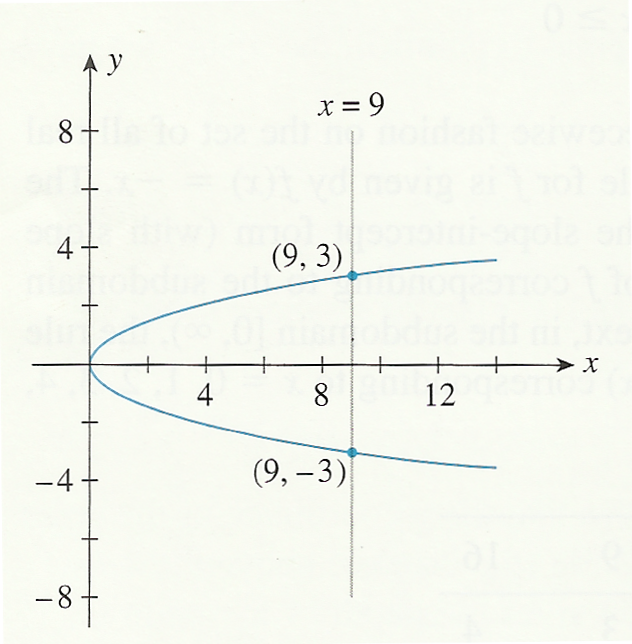
\includegraphics[scale=1]{./fgraph-03.png}
  \end{figure}
\end{frame}

\begin{frame}
  \frametitle{Vertical Line Test Exercise}
In the next four slides, determine which graphs correspond to a function.
\end{frame}

\begin{frame}
  \frametitle{Vertical Line Test Exercise I}
  \begin{figure}[h]
    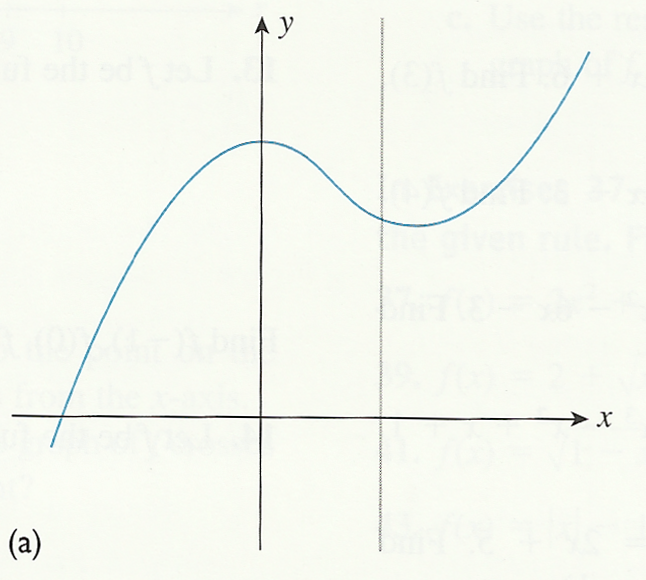
\includegraphics[scale=1]{./vertical-01.png}
  \end{figure}
\end{frame}

\begin{frame}
  \frametitle{Vertical Line Test Exercise II}
  \begin{figure}[h]
    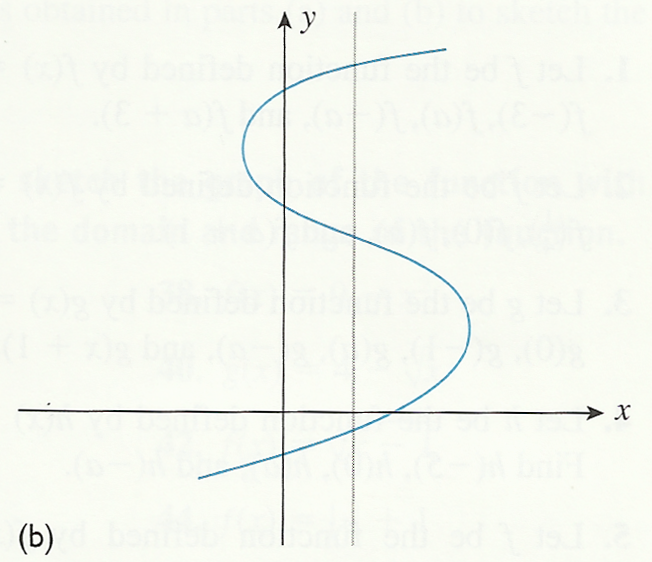
\includegraphics[scale=1]{./vertical-02.png}
  \end{figure}
\end{frame}

\begin{frame}
  \frametitle{Vertical Line Test Exercise III}
  \begin{figure}[h]
    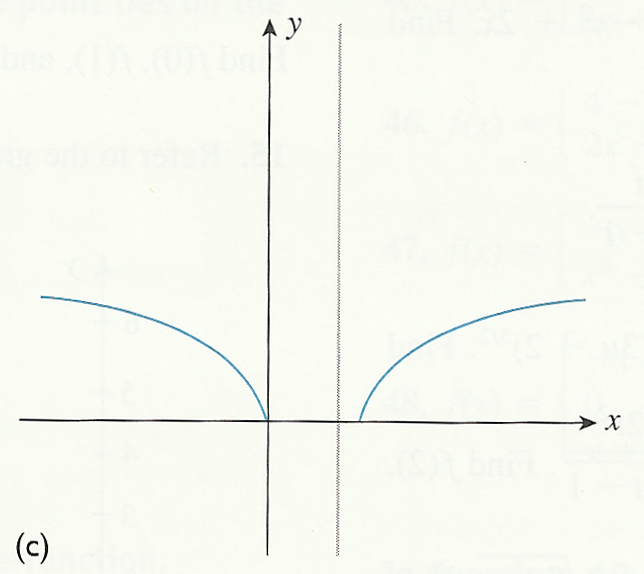
\includegraphics[scale=1]{./vertical-03.png}
  \end{figure}
\end{frame}

\begin{frame}
  \frametitle{Vertical Line Test Exercise IV}
  \begin{figure}[h]
    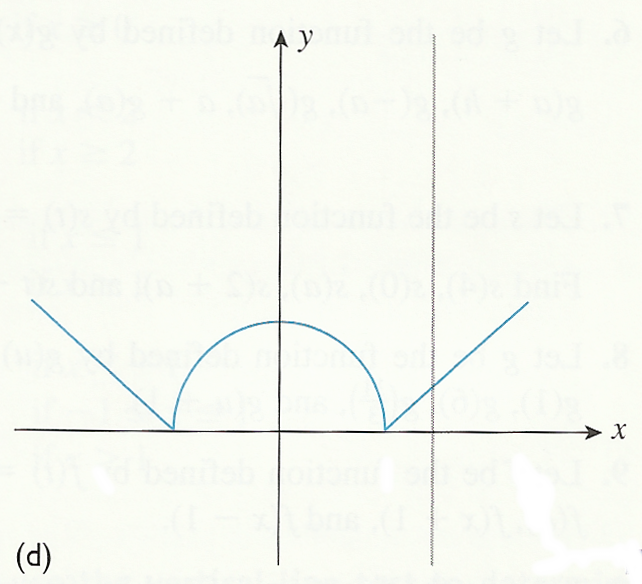
\includegraphics[scale=1]{./vertical-04.png}
  \end{figure}
\end{frame}

\begin{frame}
  \frametitle{Function Algebra}
Let $f$ and $g$ be functions with domain $A$ and $B$, respectively.
Then the \alert{sum} $f+g$, \alert{difference} $f-g$, and
\alert{product} $fg$ of $f$ and $g$ are functions with domain
$A\cap{}B$ (the intersection of $A$ and $B$) and rule given by
\begin{equation}
  \label{eq:maichong}
  (f+g)(x)=f(x)+g(x)
\end{equation}
\begin{equation}
  \label{eq:pieshouz}
  (f-g)(x)=f(x)-g(x)
\end{equation}
\begin{equation}
  \label{eq:queebeih}
  (fg)(x)=f(x)\cdot{}g(x)
\end{equation}
The \alert{quotient} $f/g$ of $f$ and $g$ has domain $A\cap{}B$
excluding all points $x$ such that $g(x)=0$ and rule given by
\begin{equation}
  \label{eq:thaochao}
  \left(\frac{f}{g}\right)(x)=\frac{f(x)}{g(x)}
\end{equation}
\end{frame}

\begin{frame}
  \frametitle{Function Composition}
Let $f$ and $g$ be functions. Then the \alert{composition} of $g$ and $f$ is
the function $g\circ{}f$ defined by
\begin{equation}
  \label{eq:aphiepae}
  (g\circ{}f)(x)=g(f(x))
\end{equation}
The domain of $g\circ{}f$ is the set of all $x$ in the domain of $f$
such that $f(x)$ lies in the domain of $g$.

\medskip

Consider the following two functions, $f(x)=\sqrt{x}$ and
  $g(y)=y-2$. What are the maximal domains in the real numbers of
  $f\circ{}g$ and $g\circ{}f$?
\end{frame}

\begin{frame}
  \frametitle{Limits Introduction}
Consider the function graph of the following function.
\begin{equation}
  \label{eq:quiekong}
  f(x)=\frac{x^{2}-1}{x-1}
\end{equation}
It looks like it is a linear equation! However, at $x=1$, $f(x)$ is
not defined. To fill the hole, we define the limit
\begin{equation}
  \label{eq:vaineiro}
  \lim_{x\rightarrow{}a}f(x)=w\mbox{ if and only if }w=L=R
\end{equation}
where $L$ is the number that the function $f$ approaches as $x$ gets
closer to $a$ with $x<a$ (that means $x\neq{}a$!); and $R$ is the
number that the function $f$ approaches as $x$ gets closer to $a$ with
$x>a$. Note: for a mathematically rigorous definition of what
``approaching'' and ``getting closer'' means we would need to
talk about sequences and series, which is a topic we won't cover here.
\end{frame}

\begin{frame}
  \frametitle{Indeterminate Form I}
Notice that
\begin{equation}
  \label{eq:iicheeci}
  f(x)=\frac{x^{2}-1}{x-1}\overset{x=1}{=}\frac{0}{0}
\end{equation}
We call this an \alert{indeterminate form}.
\end{frame}

\begin{frame}
  \frametitle{Indeterminate Form}
Notice that except at $x=1$
\begin{equation}
  \label{eq:dooshool}
  f(x)=\frac{x^{2}-1}{x-1}=\frac{\cancel{(x-1)}(x+1)}{\cancel{x-1}}=x+1=g(x)
\end{equation}
$f$ and $g$ agree everywhere except on $x=1$. Consider the following
rule,
\begin{block}{One Disagreement Rule}
If $f=g$ except in one point, then
$\lim_{x\rightarrow{}a}f(x)=\lim_{x\rightarrow{}a}g(x)$ for all $a$,
even the $a$ where $f$ and $g$ disagree.
\end{block}
Therefore
\begin{equation}
  \label{eq:eengemia}
  \lim_{x\rightarrow{}1}\frac{x^{2}-1}{x-1}=\lim_{x\rightarrow{}1}(x+1)=2
\end{equation}
\end{frame}

\begin{frame}
  \frametitle{Continuity}
Consider a simple function like $f(x)=x^{3}$. What is
$\lim_{x\rightarrow{}4}f(x)$? The answer is almost trivial,
\begin{equation}
  \label{eq:iepeacha}
  \lim_{x\rightarrow{}4}f(x)=f(4)=4^{3}=64
\end{equation}
Why is this true? Because $f$ is continuous at $x=4$. There are no
holes, jumps, gaps, or breaks of the function graph at $x=4$. 
% In fact,
% $f$ is continuous on the whole domain of $f$. A function is
% \alert{continuous} at $x=a$ if and only if (1) $f(a)$ is defined; (2)
% $\lim_{x\rightarrow{}a}f(x)$ exists; and (3)
% $\lim_{x\rightarrow{}a}f(x)=f(a)$. 
Constant functions, the identity
function, linear functions, polynomial functions, 
exponential and logarithmic functions are all continuous. Rational
functions and other functions are sometimes \alert{not} continuous.
\end{frame}

\begin{frame}
  \frametitle{Interesting Cases}
  A function is continuous if and only if
  $\lim_{x\rightarrow{}c}=f(c)$. This means that (i) the function
  needs to be defined at $x=c$; (ii) the limit needs to be defined at
  $x=c$; and (iii) the function value and the limit need to be equal
  to each other.

Consider the following interesting cases:
\begin{enumerate}
\item<1-> A function that is continuous and well defined at $x=a$.
\item<2-> A function that is not continuous at $x=a$.
\item<3-> A function where the limit exists but $\lim_{x\rightarrow{}c}\neq{}f(c)$.
\item<4-> A function such as $f(x)=\sin(1/x)$.
\end{enumerate}
\end{frame}

% \begin{frame}
%   \frametitle{Informal Definition of Limit}
% The function $f$ has the \alert{limit} $L$ as $x$ approaches $a$,
% written
% \begin{equation}
%   \label{eq:beiquoob}
%   \lim_{x\rightarrow{}a}f(x)=L
% \end{equation}
% if the value of $f(x)$ can be made as close to the number $L$ as we
% please by taking $x$ sufficiently close to (but not equal to) $a$.
% \end{frame}

\begin{frame}
  \frametitle{No Limit Examples I}
  \begin{figure}[h]
    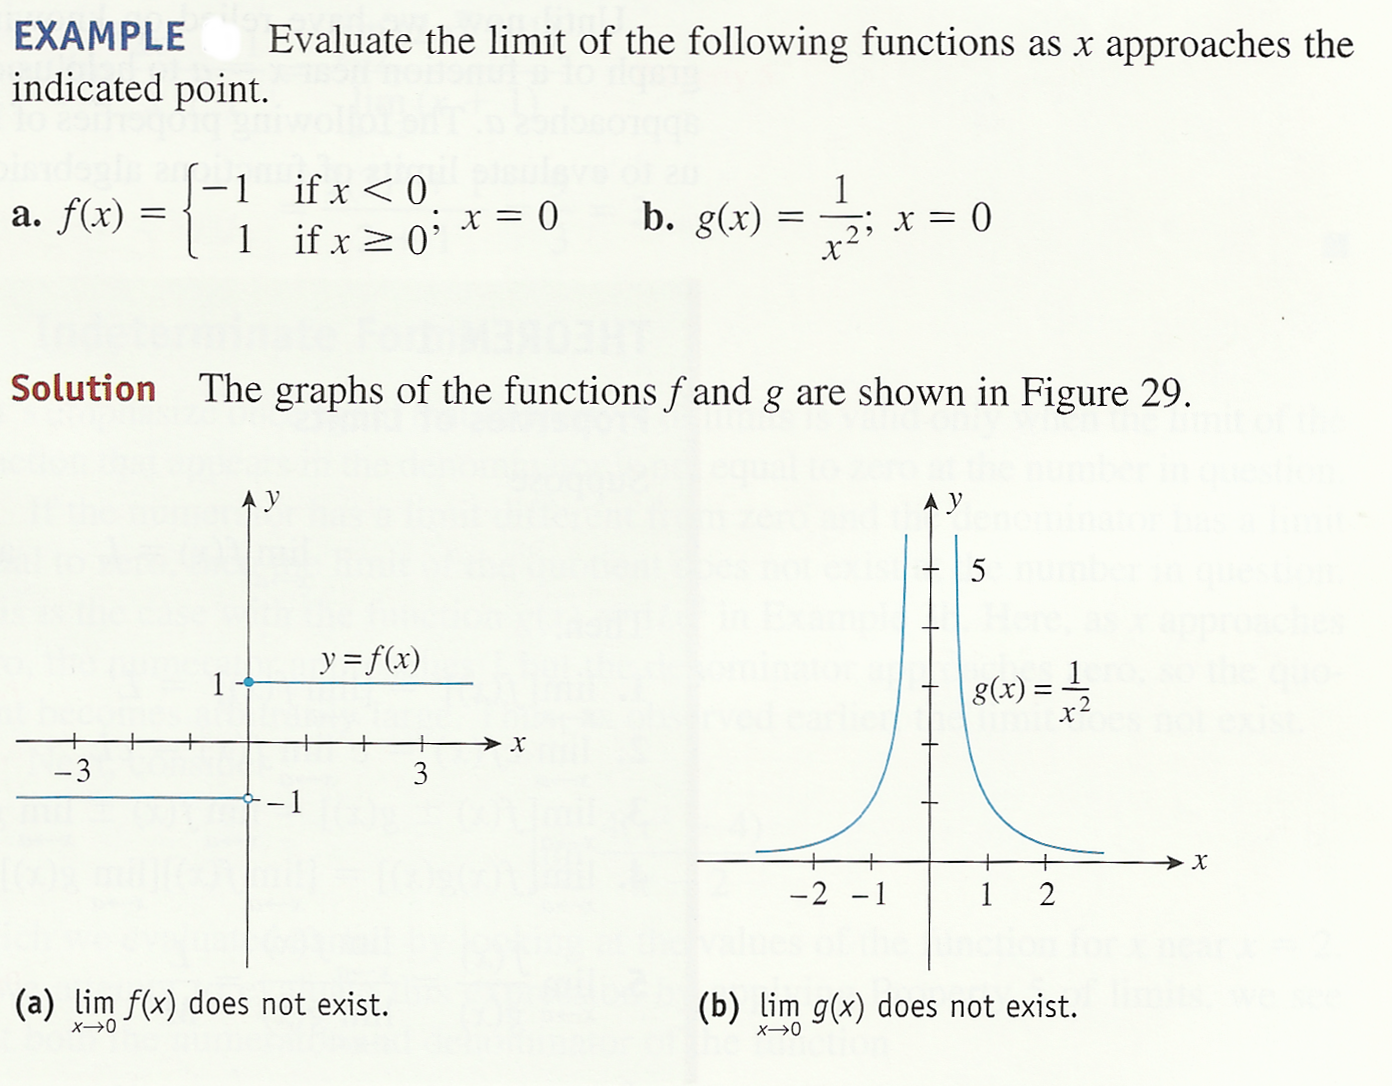
\includegraphics[scale=.9]{./limita.png}
  \end{figure}
\end{frame}

\begin{frame}
  \frametitle{No Limit Example II}
  \begin{figure}[h]
    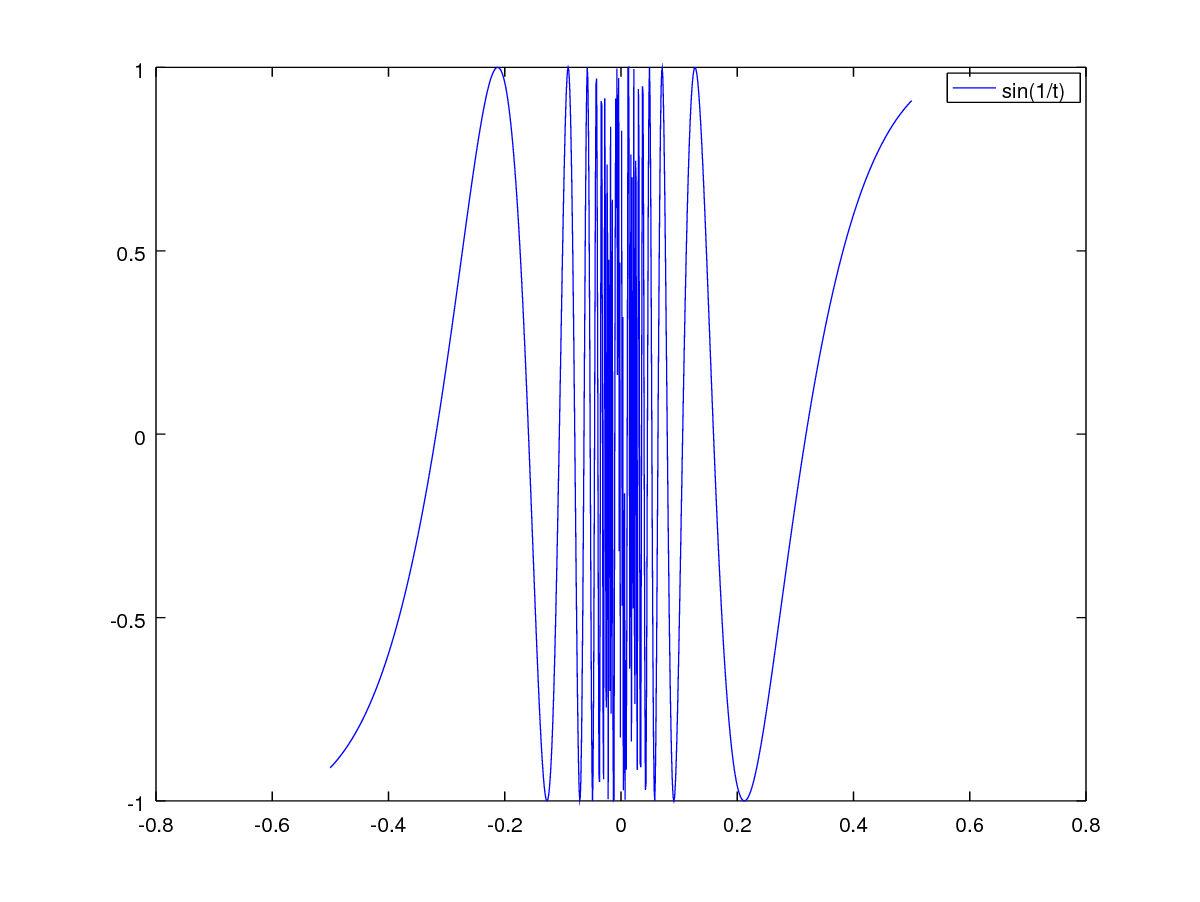
\includegraphics[scale=.5]{./sineoneoverx.png}
  \end{figure}
\end{frame}

\begin{frame}
  \frametitle{Properties of Limits}
  Suppose $\lim_{x\rightarrow{}a}f(x)=L$ and
  $\lim_{x\rightarrow{}a}g(x)=M$. Then (call this \alert{Theorem 1}),
\begin{equation}
  \label{eq:johvoohu}
  \lim_{x\rightarrow{}a}[f(x)]^{r}=L^{r},r\mbox{ a real number}
\end{equation}
\begin{equation}
  \label{eq:eeyootoh}
  \lim_{x\rightarrow{}a}[c\cdot{}f(x)]=c\cdot{}L,c\mbox{ a real number}
\end{equation}
\begin{equation}
  \label{eq:kohzahwa}
  \lim_{x\rightarrow{}a}[f(x)\pm{}g(x)]=L\pm{}M
\end{equation}
\begin{equation}
  \label{eq:aekaqued}
  \lim_{x\rightarrow{}a}[f(x)g(x)]=LM
\end{equation}
\begin{equation}
  \label{eq:ahkeigae}
  \lim_{x\rightarrow{}a}\frac{f(x)}{g(x)}=\frac{L}{M},\mbox{provided that }M\neq{}0
\end{equation}
\end{frame}

\begin{frame}
  \frametitle{Properties of Limits Exercises}
Use the properties of limits to evaluate the following,
\begin{equation}
  \label{eq:eemoopha}
 \lim_{x\rightarrow{}2}x^{3} 
\end{equation}
\begin{equation}
  \label{eq:queebaet}
 \lim_{x\rightarrow{}4}5x^{3/2} 
\end{equation}
\begin{equation}
  \label{eq:xoquaenu}
 \lim_{x\rightarrow{}1}\left(5x^{4} -2\right)
\end{equation}
\begin{equation}
  \label{eq:othahzau}
 \lim_{x\rightarrow{}3}2x^{3}\sqrt{x^{2}+7}
\end{equation}
\begin{equation}
  \label{eq:ayaivoma}
 \lim_{x\rightarrow{}2}\frac{2x^{2}+1}{x+1}
\end{equation}
\end{frame}

\begin{frame}
  \frametitle{Another Indeterminate Form Example I}
  Here is an example where by skillful manipulation we can determine
  the limit even though at first the limit is in indeterminate form.
  Let
\begin{equation}
  \label{eq:xierigai}
  f(x)=\frac{\sqrt{1+x}-1}{x}
\end{equation}
What is $\lim_{x\rightarrow{}0}f(x)$? If we leave the fraction
unchanged, it will give us an indeterminate form. However, if we
multiply both numerator and denominator by $(\sqrt{1+x}+1)$, we avoid
the indeterminate form!
\begin{equation}
  \label{eq:ciabohmi}
  \lim_{x\rightarrow{}0}f(x)=\lim_{x\rightarrow{}0}\frac{\sqrt{1+x}-1}{x}=\lim_{x\rightarrow{}0}\frac{1}{\sqrt{1+x}+1}=\frac{1}{\sqrt{1}+1}=\frac{1}{2}
\end{equation}
Look at the function graph of $f(x)$ to verify that this is the
correct limit.
\end{frame}

\begin{frame}
  \frametitle{Another Indeterminate Form Example II}
  \begin{figure}[h]
    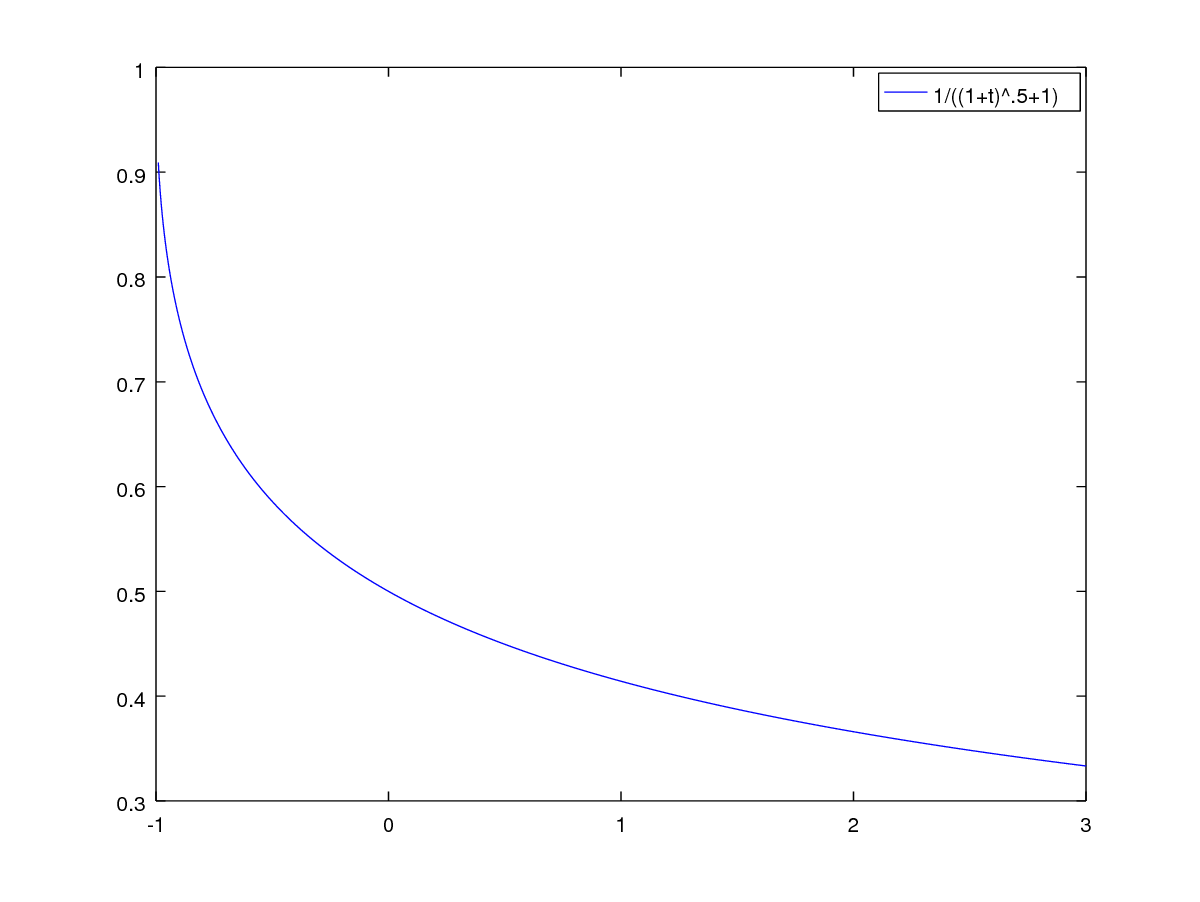
\includegraphics[scale=.5]{./indeterminate.png}
  \end{figure}
\end{frame}

\begin{frame}
  \frametitle{Limits at Infinity I}
Sometimes, we want to know what happens to a function graph when
either $x$ or $-x$ get very large. We use the infinity sign $\infty$
for notation, but note that we do NOT use infinity to define these
limits. 
\begin{equation}
  \label{eq:xetieshe}
  \lim_{x\rightarrow{}\infty}f(x)=w\mbox{ if and only if }w=S
\end{equation}
where $S$ is a number such that for any tiny number $\varepsilon$
there is a real number $x_{0}$ and
$\vert{}f(x)-S\vert<\varepsilon$ for all $x>x_{0}$.
\end{frame}

\begin{frame}
  \frametitle{Limits at Infinity II}
% Sometimes, we want a limit not at $x=a$ but as $x$ goes to positive or
% negative infinity (i.e.\ increases or decreases without bound). We use
% the symbol $\infty$ for infinity. 
For example, what is
\begin{equation}
  \label{eq:wingeisa}
  \lim_{x\rightarrow\infty}\frac{2x^{2}}{1+x^{2}}
\end{equation}
or
\begin{equation}
  \label{eq:ahxaibah}
  \lim_{x\rightarrow{}-\infty}\frac{2x^{2}}{1+x^{2}}
\end{equation}
\end{frame}

\begin{frame}
  \frametitle{Limits at Infinity III}
  \begin{figure}[h]
    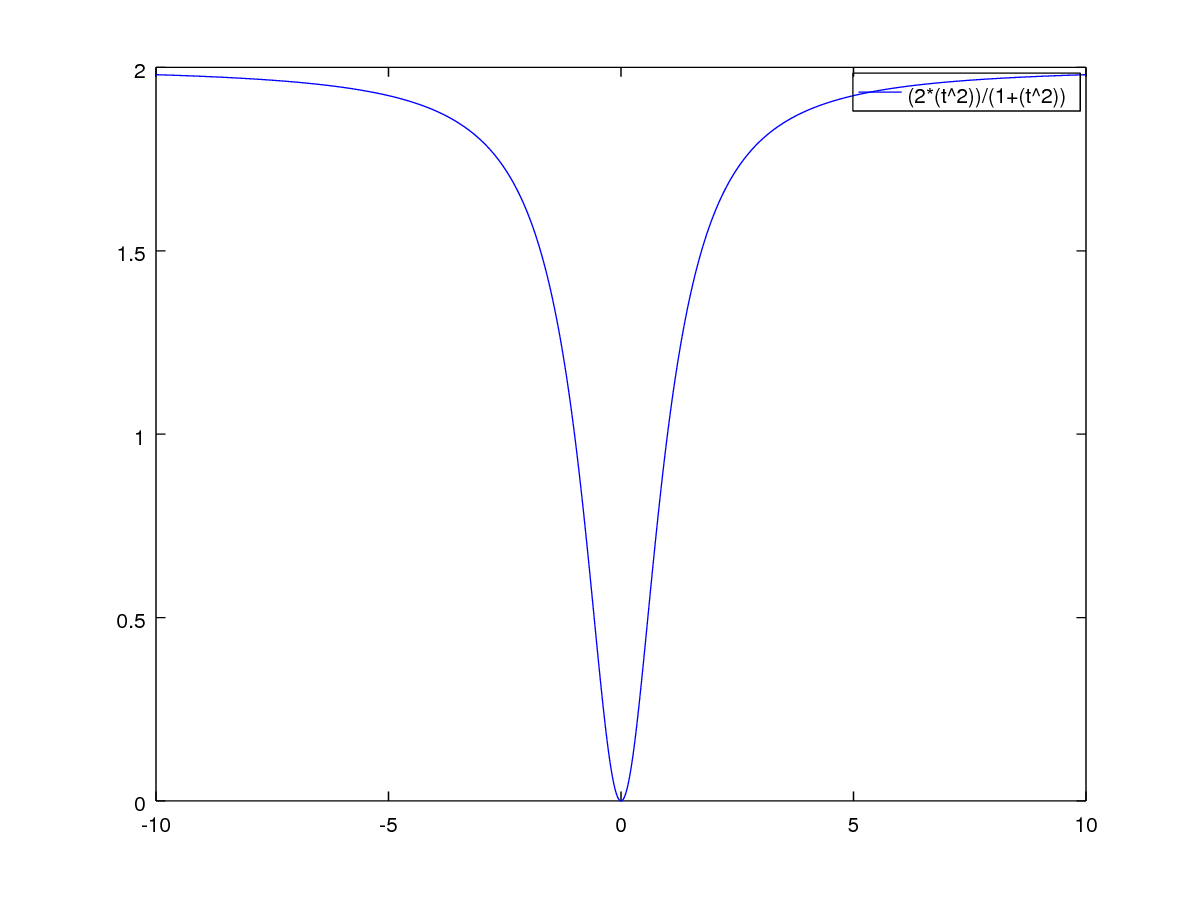
\includegraphics[scale=.5]{./lai.png}
  \end{figure}
\end{frame}

\begin{frame}
  \frametitle{Limits at Infinity IV}
Here is another important property of limits (call this \alert{Theorem
2}). If $1/x^{n}$ is defined and $n>0$, then
\begin{equation}
  \label{eq:faingiej}
  \lim_{x\rightarrow{}\infty}\frac{1}{x^{n}}=0\mbox{ and }\lim_{x\rightarrow{}-\infty}\frac{1}{x^{n}}=0
\end{equation}
\end{frame}

\begin{frame}
  \frametitle{Polynomial and Rational Functions}
A polynomial function looks like this,
\begin{equation}
  \label{eq:kaimeeyo}
  p(x)=a_{n}x^{n}+a_{n-1}x^{n-1}+\ldots{}+a_{2}x^{2}+a_{1}x+a_{0}
\end{equation}
For example, $p(x)=7x^{3}-4.7x^{2}+6$. $n>0$ is a natural number, and
the $a_{i}$ are called \alert{coefficients}. They are real numbers.
A rational function looks like this,
\begin{equation}
  \label{eq:raephoot}
  q(x)=\frac{p_{1}(x)}{p_{2}(x)}
\end{equation}
where $p_{1}(x)$ and $p_{2}(x)$ are polynomial functions. For example,
\begin{equation}
  \label{eq:yaingiaj}
  q(x)=\frac{5x^{2}-\pi{}x+9000}{e^{2}x+2}
\end{equation}
\end{frame}

\begin{frame}
  \frametitle{Limits at Infinity V}
When we are looking for the limit of rational functions as they go to
negative or positive infinity, we often get an indeterminate form.
\begin{equation}
  \label{eq:airoovae}
  \lim_{x\rightarrow\infty}\frac{x^{2}-x+3}{2x^{3}+1}=\frac{\infty}{\infty}
\end{equation}
Here is a technique that will almost always work. Divide both the
numerator and the denominator by $x^{m}$, where $m$ is the highest
exponent you can find.
\begin{equation}
  \label{eq:ahrahnei}
  \lim_{x\rightarrow\infty}\frac{x^{2}-x+3}{2x^{3}+1}=\lim_{x\rightarrow\infty}\frac{\frac{1}{x}-\frac{1}{x^{2}}+\frac{3}{x^{3}}}{2+\frac{1}{x^{3}}}=\frac{0}{2}=0
\end{equation}
\end{frame}

\begin{frame}
  \frametitle{Limits at Infinity VI}
Here are two more examples.
\begin{equation}
  \label{eq:ikiegeip}
  \lim_{x\rightarrow{}-\infty}\frac{3x^{2}+8x-4}{2x^{2}+4x-5}=\lim_{x\rightarrow{}-\infty}\frac{3-\frac{8}{x}-\frac{4}{x^{2}}}{2+\frac{4}{x}-\frac{5}{x^{2}}}=\frac{3}{2}=1.5
\end{equation}
\begin{equation}
  \label{eq:deegiech}
  \lim_{x\rightarrow{}\infty}\frac{2x^{3}-3x^{2}+1}{x^{2}+2x+4}=\lim_{x\rightarrow{}\infty}\frac{2-\frac{3}{x}+\frac{1}{x^{3}}}{\frac{1}{x}+\frac{2}{x^{2}}+\frac{4}{x^{3}}}=\frac{2}{0}=\mbox{undefined}
\end{equation}
In the second example, the limit does not exist. Sometimes, we write
$\lim_{x\rightarrow{}a}=\infty$ or $\lim_{x\rightarrow{}a}=-\infty$,
depending on which way the function goes.
\end{frame}

\begin{frame}
  \frametitle{Example I}
Consider the function,
\begin{equation}
  \label{eq:shuungae}
  f(x)=\frac{x-4}{\sqrt{x}-2}
\end{equation}
Let's find
\begin{equation}
  \label{eq:ailuiquo}
  \lim_{x\rightarrow{}4}f(x)
\end{equation}
\end{frame}

\begin{frame}
  \frametitle{Example II}
First, fill out the table:

\begin{tabular}{|l|l|l|l|}\hline
  $x=3$ & $f(x)= 3.7321$ & $x=5$ & $f(x)=4.2361$ \\ \hline
  $x=3.5$ & & $x=4.5$ &  \\ \hline
  $x=3.75$ & & $x=4.25$ & \\ \hline
  $x=3.9$ &  & $x=4.1$ & \\ \hline
  $x=3.95$ & & $x=4.05$ & \\ \hline
  $x=3.99$ & & $x=4.01$ & \\ \hline
\end{tabular}
\end{frame}

\begin{frame}
  \frametitle{Example III}
Next, let's assume that $x\neq{}4$ and expand both the numerator
and denominator by $\sqrt{x}+2$. Simplify
\begin{equation}
  \label{eq:oudiolee}
  g(x)=\frac{(x-4)\cdot(\sqrt{x}+2)}{(\sqrt{x}-2)\cdot(\sqrt{x}+2)}\mbox{ on domain }\mathbb{R}\setminus\{4\}
\end{equation}
Except on $x=4$, $g$ agrees with $f$. Determine
$\lim_{x\rightarrow{}4}g(x)$.
\end{frame}

\begin{frame}
  \frametitle{Exercises I}
Evaluate the following two limits.
\begin{equation}
  \label{eq:uheafaix}
  \lim_{x\rightarrow{}3}=\frac{\sqrt{x^{2}+7}+\sqrt{3x-5}}{x+2}
\end{equation}
\begin{equation}
  \label{eq:azeeghee}
  \lim_{x\rightarrow{}-1}\frac{x^{2}-x-2}{2x^{2}-x-3}
\end{equation}
\end{frame}

\begin{frame}
  \frametitle{Exercises II}
Evaluate the following three limits.
\begin{equation}
  \label{eq:haeceema}
  \lim_{x\rightarrow{}2}3
\end{equation}
\begin{equation}
  \label{eq:aogedish}
  \lim_{x\rightarrow\infty}\frac{3x+2}{x-5}
\end{equation}
\begin{equation}
  \label{eq:xaebiaph}
  \lim_{x\rightarrow\infty}\frac{x^{5}-x^{3}+x-1}{x^{6}+2x^{2}+1}
\end{equation}
\end{frame}

\begin{frame}
  \frametitle{Finding Limits Exercises}
Find the following limits,
\begin{equation}
  \label{eq:ixahngoo}
\lim_{x\rightarrow{}9}\frac{\sqrt{x}-3}{x-9}
\end{equation}
\begin{equation}
  \label{eq:etheshoh}
\lim_{x\rightarrow\infty}\frac{\sqrt{x^{2}-8x}}{2x+1}
\end{equation}
\begin{equation}
  \label{eq:chahgaew}
\lim_{x\rightarrow{}-1}\frac{x^{2}-x-2}{2x^{2}-x-3}
\end{equation}
\begin{equation}
  \label{eq:oofeegae}
\lim_{x\rightarrow\infty}\frac{2+\frac{1}{x+4}}{3-\frac{1}{x^{2}}}
\end{equation}
\begin{equation}
  \label{eq:yupeethi}
\lim_{x\rightarrow\infty}\frac{x-2x^{3}}{(1+x)^{3}}
\end{equation}
\begin{equation}
  \label{eq:reibaize}
\lim_{x\rightarrow\infty}\frac{\sqrt{4x^{2}+3}}{x+5}
\end{equation}
\end{frame}

\begin{frame}
In Einstein's theory of relativity, the length $L$ of an object moving
at a velocity $v$ is 
\begin{equation}
  \label{eq:aumiepha}
L=L_{0}\sqrt{1-\frac{v^{2}}{c^{2}}}
\end{equation}
where $c$ is the speed of light and $L_{0}$ is the length of the
object at rest. What is the one-sided limit of $L$ as $v$ gets
faster and faster?
\end{frame}

\begin{frame}
  \frametitle{Introduction to Calculus}
\alert{Calculus} solves many problems for which it was not originally
designed. The initial motivation for calculus was to find the slope of
a tangent on a curve and the area of a region bounded by a curve.
  \begin{figure}[h]
    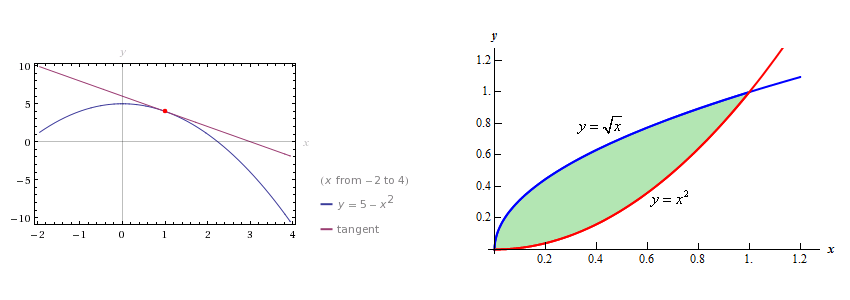
\includegraphics[scale=.35]{./regiontangent.png}
  \end{figure}
\end{frame}

\begin{frame}
  \frametitle{A Real-Life Example I}
Consider a magnetic levitation train accelerating on a straight
monorail track. The position of the train (in feet) from the origin at
time $t$ is given by
\begin{equation}
  \label{eq:pupibahk}
  s=f(t)=4t^{2}
\end{equation}
What is the velocity of the train at $t=2$?
\end{frame}

\begin{frame}
  \frametitle{A Real-Life Example II}
It appears to make sense only if we calculate the velocity given an
interval of time rather than just one point in time. For example, the
velocity between $t=2$ and $t=3$ is 
\begin{equation}
  \label{eq:einohkie}
  v_{[2,3]}=\frac{f(3)-f(2)}{3-2}=20
\end{equation}
More generally,
\begin{equation}
  \label{eq:phaedais}
  v_{[2,t]}=g(t)=\frac{f(t)-f(2)}{t-2}=\frac{4(t^{2}-4)}{t-2}
\end{equation}
$g$ is not defined at $t=2$, but it is defined all around $t=2$, so we
can ask ourselves the question: what happens when $t\rightarrow{}2$
from below; or when $t\rightarrow{}2$ from above? It turns out that
either way, the number approaches 16.
\end{frame}

\begin{frame}
  \frametitle{Velocity at a Point}
  Now remember formula (\ref{eq:phaedais}) from a few slides ago.
\begin{displaymath}
  v_{[2,t]}=g(t)=\frac{f(t)-f(2)}{t-2}=\frac{4(t^{2}-4)}{t-2}
\end{displaymath}
If we found the limit as $t\rightarrow{}2$, it would serve as an
intuitive definition of what a velocity is at a point (instead of on
an interval). Unfortunately, the limit has the \alert{indeterminate
  form}
\begin{equation}
  \label{eq:toochoir}
  \lim_{t\rightarrow{}2}\frac{4(t^{2}-4)}{t-2}=\frac{0}{0}
\end{equation}
However, notice that for $t\neq{}2$,
\begin{equation}
  \label{eq:geeshaiz}
  g(t)=\frac{4(t^{2}-4)}{t-2}=\frac{4(t+2)\cancel{(t-2)}}{\cancel{t-2}}=4(t+2)
\end{equation}
\end{frame}

\begin{frame}
  \frametitle{Tangent Lines I}
Remember our magnetic levitation train. The distance-time function was
\begin{equation}
  \label{eq:leezaach}
  s=f(t)=4t^{2}
\end{equation}
The velocity of the train over a given interval is
\begin{equation}
  \label{eq:ohgheith}
  v_{[t_{1},t_{2}]}=\frac{f(t_{2})-f(t_{1})}{t_{2}-t_{1}}
\end{equation}
This velocity is also the slope of the line going through the two
function values $f(t_{1})$ and $f(t_{2})$. We call such a line a
\alert{secant line}. 
\end{frame}

\begin{frame}
  \frametitle{Tangent Lines II}
  Now imagine $t_{1}$ and $t_{2}$ moving closer and closer together at
  a point $a$ (for the train, we used $a=2$). If both of these limits
  exist and agree with each other, we have a velocity at a point,
\begin{equation}
  \label{eq:aixohshi}
  \lim_{t\rightarrow{}a}v_{[a,t]}\mbox{ for }t>a
\end{equation}
\begin{equation}
  \label{eq:oongahgh}
  \lim_{t\rightarrow{}a}v_{[t,a]}\mbox{ for }t<a
\end{equation}
This velocity at a point is also the slope of the line that just
touches the function graph without crossing it. We call it a
\alert{tangent line} at $t=a$. The slope of the tangent line is
sometimes also called the \alert{rate of change}.
\end{frame}

\begin{frame}
  \frametitle{Tangent Lines III}
  Think of a tangent line as the limit of secant lines. The slope of a
  tangent line at a point $P=(x,f(x))$, if it exists, is
\begin{equation}
  \label{eq:cheevooj}
  \lim_{h\rightarrow{}0}\frac{f(x+h)-f(x)}{h}
\end{equation}
  \begin{figure}[h]
    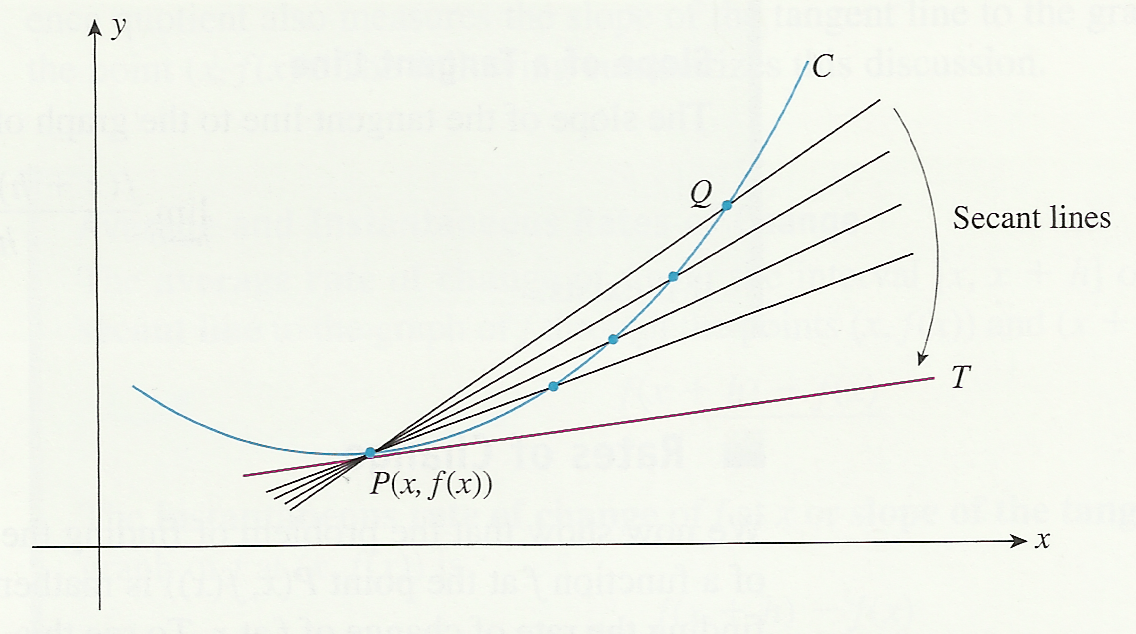
\includegraphics[scale=.7]{./tangent1.png}
  \end{figure}
\end{frame}

\begin{frame}
  \frametitle{Tangent Lines IV}
  Think of a tangent line as the limit of secant lines. The slope of a
  tangent line at a point $P=(x,f(x))$, if it exists, is
\begin{equation}
  \label{eq:faiseeth}
  \lim_{h\rightarrow{}0}\frac{f(x+h)-f(x)}{h}
\end{equation}
  \begin{figure}[h]
    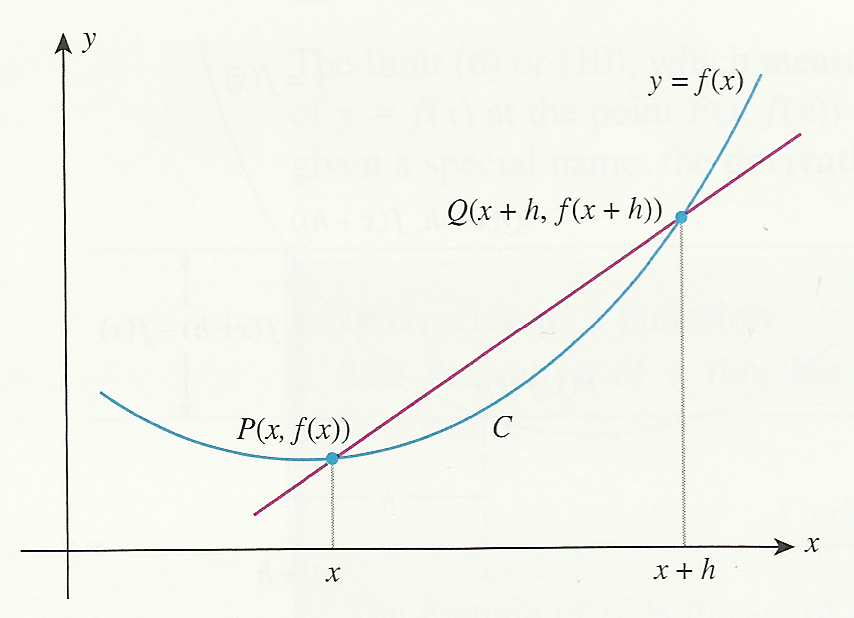
\includegraphics[scale=.7]{./tangent2.png}
  \end{figure}
\end{frame}

\begin{frame}
  \frametitle{Derivatives}
The derivative of a function $f$ with respect to $x$ is the function
$f'$ (read ``$f$ prime''),
\begin{equation}
  \label{eq:lohfasoe}
f'(x)=\lim_{h\rightarrow{}0}\frac{f(x+h)-f(x)}{h}
\end{equation}
The domain of $f'$ is the set of all $x$ where the limit exists.
\end{frame}

\begin{frame}
  \frametitle{Derivatives Diagram I}
  \begin{figure}[h]
    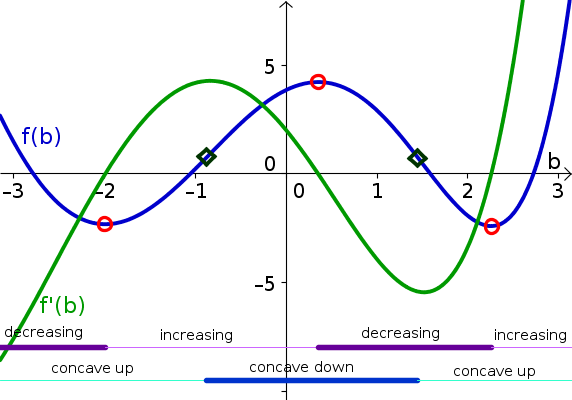
\includegraphics[scale=1.8]{./derivs2.png}
  \end{figure}
\end{frame}

\begin{frame}
  \frametitle{Derivatives Diagram II}
  \begin{figure}[h]
    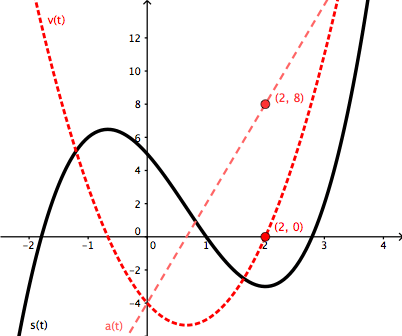
\includegraphics[scale=.6]{./derivs1.png}
  \end{figure}
\end{frame}

\begin{frame}
  \frametitle{Basic Rules of Differentiation I}
  \begin{block}{Rule 1}
Derivative of a Constant
  \end{block}
\begin{equation}
  \label{eq:ligoovah}
f'(x)=0\mbox{ for }f(x)=c
\end{equation}
Reason:
\begin{equation}
  \label{eq:ahnieluz}
f'(x)=\lim_{h\rightarrow{}0}\frac{f(x+h)-f(x)}{h}=\lim_{h\rightarrow{}0}\frac{c-c}{h}=\lim_{h\rightarrow{}0}0=0
\end{equation}
\end{frame}

\begin{frame}
  \frametitle{Basic Rules of Differentiation II}
  \begin{block}{Rule 2}
The Power Rule
  \end{block}
\begin{equation}
  \label{eq:oomaenee}
f'(x)=nx^{n-1}\mbox{ for }f(x)=x^{n}
\end{equation}
Reason (the general case is messy, we will just show it for $f(x)=x^{2}$):
\begin{equation}
  \label{eq:eeyeejeu}
f'(x)=\lim_{h\rightarrow{}0}\frac{f(x+h)-f(x)}{h}=\lim_{h\rightarrow{}0}\frac{(x+h)^{2}-x^{2}}{h}=\notag
\end{equation}
\begin{equation}
  \label{eq:wuuxaise}
\lim_{h\rightarrow{}0}\frac{2xh+h^{2}}{h}=\lim_{h\rightarrow{}0}(2x+h)=2x
\end{equation}
\end{frame}

\begin{frame}
  \frametitle{Basic Rules of Differentiation III}
  \begin{block}{Rule 3}
Derivative of a Constant Multiple of a Function
  \end{block}
\begin{equation}
  \label{eq:thahchae}
g'(x)=c\cdot{}f'(x)\mbox{ for }g(x)=c\cdot{}f(x)
\end{equation}
Reason:
\begin{equation}
  \label{eq:quaipahn}
g'(x)=\lim_{h\rightarrow{}0}\frac{g(x+h)-g(x)}{h}=\lim_{h\rightarrow{}0}\frac{c\cdot{}f(x+h)-c\cdot{}f(x)}{h}=\notag
\end{equation}
\begin{equation}
  \label{eq:mitahrei}
\lim_{h\rightarrow{}0}c\cdot{}\frac{f(x+h)-f(x)}{h}=c\cdot\lim_{h\rightarrow{}0}\frac{f(x+h)-f(x)}{h}=c\cdot{}f'(x)
\end{equation}
\end{frame}

\begin{frame}
  \frametitle{Basic Rules of Differentiation IV}
  \begin{block}{Rule 4}
The Sum Rule
  \end{block}
\begin{equation}
  \label{eq:oubajaez}
g'(x)=f_{1}'(x)+f_{2}'(x)\mbox{ for }g(x)=f_{1}(x)+f_{2}(x)
\end{equation}
Reason:
\begin{equation}
  \label{eq:heyanaci}
g'(x)=\notag
\end{equation}
\begin{equation}
  \label{eq:bahgosio}
\lim_{h\rightarrow{}0}\frac{g(x+h)-g(x)}{h}=\lim_{h\rightarrow{}0}\frac{f_{1}(x+h)+f_{2}(x+h)-f_{1}(x)-f_{2}(x)}{h}=\notag
\end{equation}
\begin{equation}
  \label{eq:eceishie}
\lim_{h\rightarrow{}0}\left(\frac{f_{1}(x+h)-f_{1}(x)}{h}+\frac{f_{2}(x+h)-f_{2}(x)}{h}\right)=f_{1}'(x)+f_{2}'(x)
\end{equation}
\end{frame}

\begin{frame}
  \frametitle{Basic Differentiation Exercises I}
Find the derivatives for the following functions.
\begin{enumerate}
\item $f(x)=4x^{5}+3x^{4}-8x^{2}+x+3$
\item $f(t)=\frac{t^{2}}{5}+\frac{5}{t^{3}}$
\item $g(z)=2z-5\sqrt{z}$
\end{enumerate}

\bigskip

Find the slope and an equation of the tangent line to the graph of
$f(x)=2x+(1/\sqrt{x})$ at the point $(1,3)$.
\end{frame}

\begin{frame}
  \frametitle{Basic Differentiation Exercises II}
Find the derivatives for the following functions.
\begin{equation}
  \label{eq:ohzahcer}
  f(x)=5x^{\frac{4}{3}}-\frac{2}{3}x^{\frac{3}{2}}+x^{2}-3x+1
\end{equation}
\begin{equation}
  \label{eq:mothoofi}
f(x)=2t^{2}+\sqrt{t^{3}}
\end{equation}
\begin{equation}
  \label{eq:aiquooyo}
  f(x)=\frac{2}{x^{2}}-\frac{3}{x^{\frac{1}{3}}}
\end{equation}
\begin{equation}
  \label{eq:achaingo}
f(x)=\frac{3}{x^{3}}+\frac{4}{\sqrt{x}}+1
\end{equation}
\end{frame}

\begin{frame}
  \frametitle{End of Lesson}
Next Lesson: Product and Quotient Rule
\end{frame}

\end{document}

